\let\negmedspace\undefined
\let\negthickspace\undefined
\documentclass[journal]{IEEEtran}
\usepackage[a5paper, margin=10mm, onecolumn]{geometry}
%\usepackage{lmodern} % Ensure lmodern is loaded for pdflatex
\usepackage{tfrupee} % Include tfrupee package

\setlength{\headheight}{1cm} % Set the height of the header box
\setlength{\headsep}{0mm}     % Set the distance between the header box and the top of the text

\usepackage{gvv-book}
\usepackage{gvv}
\usepackage{cite}
\usepackage{amsmath,amssymb,amsfonts,amsthm}
\usepackage{algorithmic}
\usepackage{graphicx}
\usepackage{textcomp}
\usepackage{xcolor}
\usepackage{txfonts}
\usepackage{listings}
\usepackage{enumitem}
\usepackage{mathtools}
\usepackage{gensymb}
\usepackage{comment}
\usepackage[breaklinks=true]{hyperref}
\usepackage{tkz-euclide} 
\usepackage{listings}
% \usepackage{gvv}                                        
\def\inputGnumericTable{}                                 
\usepackage[latin1]{inputenc}                                
\usepackage{color}                                            
\usepackage{array}                                            
\usepackage{longtable}                                       
\usepackage{calc}                                             
\usepackage{multirow}                                         
\usepackage{hhline}                                           
\usepackage{ifthen}                                           
\usepackage{lscape}
\begin{document}

\bibliographystyle{IEEEtran}
\vspace{3cm}

\title{2.8.9}
\author{EE25btech11028 - J.Navya sri}
% \maketitle
% \newpage
% \bigskip
{\let\newpage\relax\maketitle}


\textbf{Question:} \\
Let $\vec{a}, \vec{b}, \vec{c}$ be three vectors such that 
$|\vec{a}|=3,\; |\vec{b}|=4,\; |\vec{c}|=5$, and each one of them is perpendicular to the sum of the other two. 
Find $|\vec{a}+\vec{b}+\vec{c}|$.

\textbf{Solution:} \\
From the identity:
\begin{equation} \label{eq1}
\mathbf{a}^\top(\mathbf{b} + \mathbf{c}) = 0,
\end{equation}
we expand:
\begin{equation} \label{eq2}
\mathbf{a}^\top \mathbf{b} + \mathbf{a}^\top \mathbf{c} = 0.
\end{equation}

Similarly, from the symmetry of dot products:
\begin{align}
\mathbf{b}^\top \mathbf{c} + \mathbf{b}^\top \mathbf{a} &= 0, \label{eq3} \\
\mathbf{c}^\top \mathbf{a} + \mathbf{c}^\top \mathbf{b} &= 0. \label{eq4}
\end{align}

Let
\begin{equation} \label{eq5}
x = \mathbf{a}^\top \mathbf{b}, \quad y = \mathbf{b}^\top \mathbf{c}, \quad z = \mathbf{c}^\top \mathbf{a}.
\end{equation}

Then equations (2), (3), and (4) become:
\begin{align}
x + z &= 0, \label{eq6} \\
x + y &= 0, \label{eq7} \\
y + z &= 0. \label{eq8}
\end{align}

\bigskip

\noindent
\textbf{Matrix Form:}  
Equations (6), (8) can be written compactly as
\[
\myvec{
1 & 0 & 1 \\
1 & 1 & 0 \\
0 & 1 & 1
}
\myvec{
x \\ y \\ z
}
=
\myvec{
0 \\ 0 \\ 0
}.
\]


Therefore:
\begin{equation} \label{eq9}
x = y = z = 0,
\end{equation}
so $\mathbf{a}, \mathbf{b}, \mathbf{c}$ are \textbf{pairwise orthogonal}.

\bigskip

The \textbf{Gram matrix} of $ (\mathbf{a}, \mathbf{b}, \mathbf{c}) $ is:
\begin{equation} \label{eq10}
G =
\myvec{
\mathbf{a}^\top \mathbf{a} & \mathbf{a}^\top \mathbf{b} & \mathbf{a}^\top \mathbf{c} \\
\mathbf{b}^\top \mathbf{a} & \mathbf{b}^\top \mathbf{b} & \mathbf{b}^\top \mathbf{c} \\
\mathbf{c}^\top \mathbf{a} & \mathbf{c}^\top \mathbf{b} & \mathbf{c}^\top \mathbf{c}
}
=
\myvec{
\|\mathbf{a}\|^2 & 0 & 0 \\
0 & \|\mathbf{b}\|^2 & 0 \\
0 & 0 & \|\mathbf{c}\|^2
}
=
\myvec{
9 & 0 & 0 \\
0 & 16 & 0 \\
0 & 0 & 25
}.
\end{equation}

Let
\[
\mathbf{u} = \myvec{1 \\ 1 \\ 1}.
\]
Then
\begin{equation} \label{eq11}
\|\mathbf{a} + \mathbf{b} + \mathbf{c}\|^2 = (\mathbf{a} + \mathbf{b} + \mathbf{c})^\top (\mathbf{a} + \mathbf{b} + \mathbf{c}) = \mathbf{u}^\top G \mathbf{u}.
\end{equation}

Now compute:
\begin{align}
\mathbf{u}^\top G \mathbf{u} 
&= \myvec{1 & 1 & 1}
\myvec{
9 & 0 & 0 \\
0 & 16 & 0 \\
0 & 0 & 25
}
\myvec{1 \\ 1 \\ 1} \nonumber \\
&= 9 + 16 + 25 = 50. \label{eq12}
\end{align}

Therefore:
\begin{equation} \label{eq13}
\|\mathbf{a} + \mathbf{b} + \mathbf{c}\| = \sqrt{50} = 5\sqrt{2}.
\end{equation}

\bigskip

\textbf{Final Answer:}
\[
\boxed{5\sqrt{2}}
\]

\textbf{Graph presentation:}
\begin{figure}[H]
\begin{center}
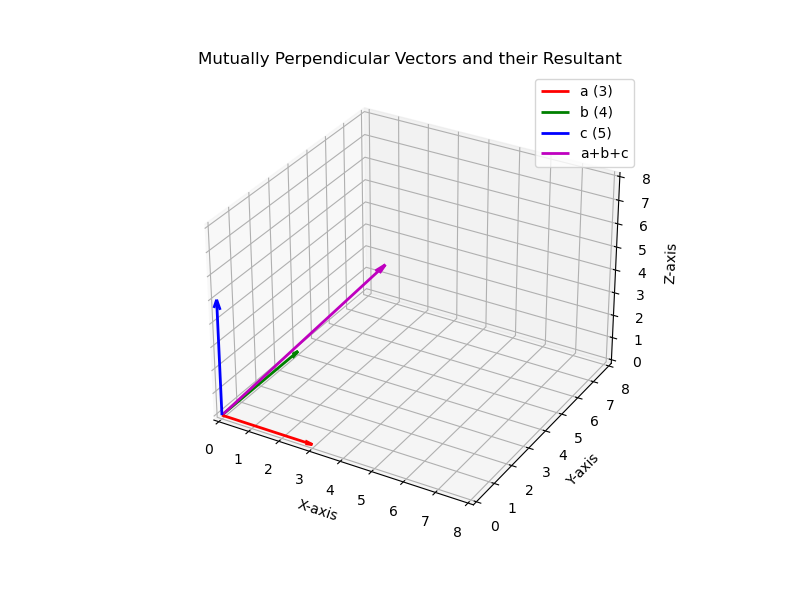
\includegraphics[width=0.6\columnwidth]{figs/fig4.png}
\end{center}
\caption{}
\label{fig:Fig}
\end{figure}    
\end{document}